\item[\textbf{3.}] \textbf{[30 min/20 puntos]} \textcolor{dkgreen}{Considera la siguiente ejecución de una implementación de una pila para tres hilos $p,q,r$ y sobre un solo objeto (de tipo pila).\\
La especificación secuencial de una pila es que el método $push(x)$ añade a $x$ al inicio de la pila y el método $pop():x$ elimina al primer elemento $x$ al inicio de la pila (mantiene LIFO). }
\begin{figure}[H]
    \centering
    \vspace{-10pt}
    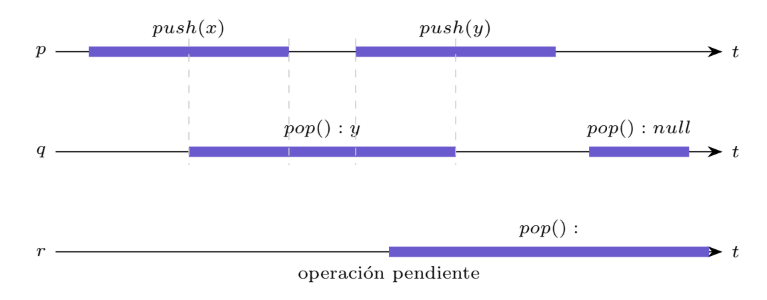
\includegraphics[width=0.8\textwidth]{Imagenes/image-1.png}
    \vspace{-10pt}
\end{figure}
\begin{enumerate}
    \item \textcolor{dkgreen}{¿Es linealizable con respecto a una pila? De ser así, incluye una linearización y especifica la \textit{extension} de $H$ y $complete(H')$.}
\end{enumerate}
Sea $H$ la ejecución (historia concurrente) de la imagen, se quiere saber si $H$ es linealizable \textbf{con respecto a una pila (estructura LIFO)}. La ejecución $H$ es linealizable si existe alguna historia secuencial legal $S$, tal que $S\equiv complete(H)$. Por lo tanto, basta que exhibamos alguna $S$ que cumpla con esto.
\par
Denotaremos que $X$ es concurrente (se traslapa) a $Y$ como $X||Y$, y denotaremos que $X$ precede a (termina antes que) $Y$ como $X<Y$. Recordemos además que:
\begin{itemize}
    \item Todo par de operaciones concurrentes entre sí, se ordenan entre ellas de la forma que más convenga, es decir, $X||Y$ es equivalente a $Y||X$.
    \item Las operaciones precedentes entre sí mantienen su ordenen la transformación, es decir que si $X<_H Y$, entonces $X <_J Y$ (con $J$ transformación de $H$).
\end{itemize}
Primero, descubramos que operaciones o tareas son concurrentes y precedentes entre sí. Las reglas que se cumplen en $H$ son:
\begin{enumerate}[label=\arabic*.]
    \item $push(x) \text{ } || \text{ } pop():y$
    \item $pop():y \text{ } || \text{ }  push(y) \text{ }  || \text{ } pop():$
    \item $pop(): \text{ }  || \text{ } pop():null$
    \item $push(x) < push(y)$
    \item $push(x) < pop():$
    \item $push(x) < pop():null$
    \item $pop():y < pop():null$
    \item $push(y) < pop():null$
\end{enumerate}
Notemos que la historia $H$ tiene una invocación pendiente: la única operación del hilo $r$ ($pop():$) no tiene respuesta. Para transformar $H$ en una historia secuencial $S$, necesitamos encontrar alguna extensión $H'$ tal que $H'=complete(H)$.
\par
Considerando todas las invocaciones completas de $H$, veamos que en algún punto $x$ y $y$ entran en la pila, y en otro punto $y$ salió de la pila, por la regla 6, 7 y 8, para que $pop():null$ solo es posible si $x$ salió de la pila. Afortunadamente, la linealizabilidad nos deja decidir si completamos o borramos las invocaciones pendientes, por lo que elegimos completar la invocación $pop():$ con una respuesta: $pop():x$. Por lo tanto, \textcolor{red}{la extensión $H'=complete(H)$} queda como:
\begin{figure}[H]
    \centering
    \vspace{-10pt}
    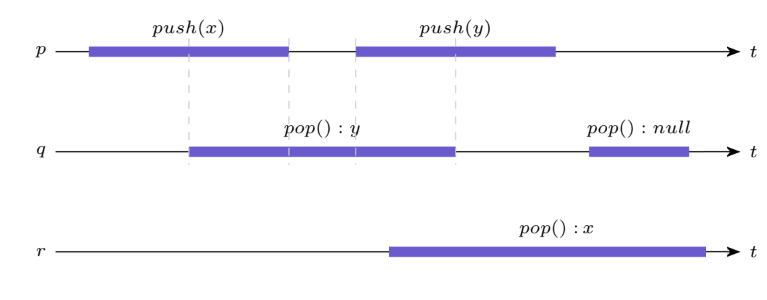
\includegraphics[width=0.8\textwidth]{Imagenes/image-3a.png}
    \vspace{-10pt}
\end{figure}
Completando y reordenando (visualmente) nuestras reglas, tenemos:
\begin{enumerate}[label=\arabic*.]
    \item $push(x) \text{ } || \text{ } pop():y$
    \item $push(y) \text{ } || \text{ }  pop():y \text{ }  || \text{ } pop():x$
    \item $pop():x \text{ }  || \text{ } pop():null$
    \item $push(x) < push(y)$
    \item $push(x) < pop():$
    \item $push(x) < pop():null$
    \item $pop():y < pop():null$
    \item $push(y) < pop():null$
\end{enumerate}
Podemos exhibir la siguiente \textcolor{red}{historia secuencial $S$}:
\begin{equation*}
    S = push(x) <push(y)<pop():y<pop(x)<pop():null
\end{equation*}
\begin{figure}[H]
    \centering
    \vspace{-10pt}
    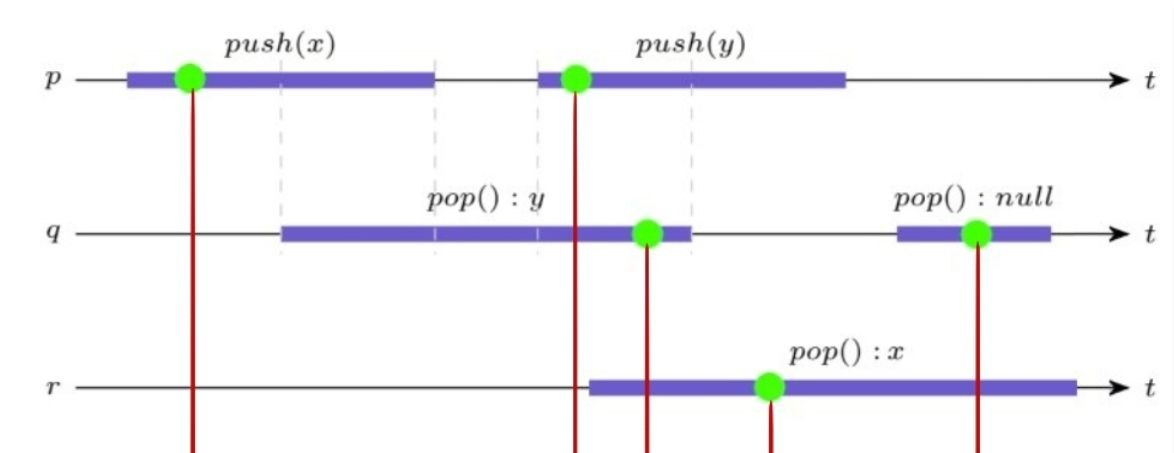
\includegraphics[width=0.8\textwidth]{Imagenes/image-3b.png}
    \vspace{-10pt}
\end{figure}
Como $S$ cumple con todas las 8 reglas de nuestras operaciones en $H'$, entonces existe $S$ una historia secuencial legal tal que $S\equiv complete(H)$.
\par
\textcolor{red}{$\therefore H$ es \textbf{linealizable} con respecto a una pila.}